\documentclass{article}
\usepackage{graphicx}

\begin{document}

\title{Répartition de ressources par homologie persistante : 
    application au développement des transports publics}
\author{Elowan}
\date{\today}

\maketitle

\section{Introduction}
L'accès aux transports publics est un enjeu majeur pour le développement des 
villes. Il est donc important de pouvoir mesurer et évaluer comment les
ressources sont réparties géographiquement afin de ne pas sous-développer
des regions de fortes densités et sur-développer celle désertes.

\section{Approche}
On récupère les données de densités de population via https://human-settlement.emergency.copernicus.eu/visualisation.php#
et de temps de trajet entre deux stations de metro via google api

\section{Persistance homologique}

La persistance homologique nous permet de détecter les trous géographiques
dans les villes. Cela nous permet de voir où il y a des zones non desservies,
des clusters de zones desservies par les transports publics. De plus, elle 
nous permet de mesurer leur persistance à différentes échelles.

Afin d'utiliser la persistance homologique, nous devons d'abord construire
un \textit{complexe simplicial} à partir des données géographiques, d'un nuage 
de points.

\textbf{Complexes simpliciaux} : Un complexe simplicial est un objet géométrique 
déterminé par une donnée combinatoire et permettant de décrire certains 
espaces topologiques en généralisant la notion de triangulation d'une surface. 
Un tel objet se présente comme un graphe avec des sommets reliés par des arêtes,
sur lesquelles peuvent se rattacher des faces triangulaires, elles-mêmes bordant 
éventuellement des faces de dimension supérieure, etc. 

A la place d'utiliser un distance basée sur la distance geodesic comme dans 
[Stable Topological Signatures for Points on 3D Shapes], nous utilisons une 
distance basée sur le temps de trajet entre deux stations. On met des points
sur les noeuds du graphe en fonction de la densités de population sur 5mn de marche 
autour

Citation : We estimate waiting times by using
Global Positioning System (GPS) ping data from mobile phones at the resource sites,
and we estimate travel times by using street-network data, per capita car-ownership
data, and the Google Maps application programming interface (API) [21]. Using these
estimates, we construct a weighted VR filtration. We weight vertices by our estimates
of waiting times, and we define the distance between two vertices to be the estimated
round-trip travel time between them. Because the weighted VR filtration is stable,
small errors in our estimates cause only small errors in the resultant PH

On considère les voisins dépendant de la filtration faite plutot qu'un rayon de taille fixe

On ne veut pas trouver de rayon tel que tous est couvert mais plutôt de quantifier
la couverture pour n'importe quel rayon choisi et connaitre la persistance de la
couverture quand on change de rayon.

D'ailleurs, dans notre problème, on ne cherche pas à étudier la relation entre
deux points (représentant des stations de métro par exemple) car n'a rien avoir 
avec l'accessibilité des ressources

Donc depuis notre nuage de points $X$, on va chercher à contruire un complexe
simplicial filtré (que l'ont appellera filtration). Une filtration est une 
suite de complexes simpliciaux imbriqués $K_0 \subset K_1 \subset \dots \subset K_n$

\begin{figure}[h!]
    \centering
    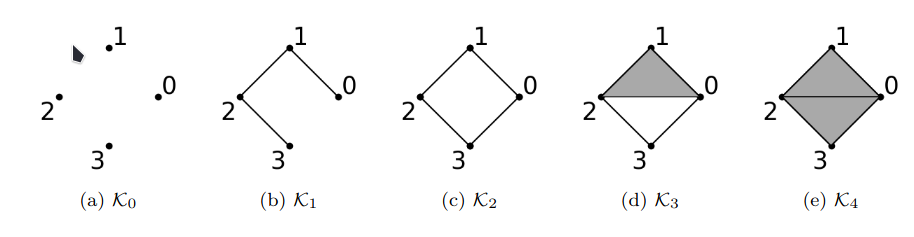
\includegraphics[width=1\textwidth]{images/Filtration ex.png}
    \caption{Filtration d'un complexe simplicial}
\end{figure}

Pour construire une filtration qui approxime un nuage de points $X = \{x_1, x_2, \dots, x_n\}$,
dans un espace métrique $(E, d)$, nous allons utiliser la filtration VR (Vietoris-Rips)
qui est une approximation de la filtration de Čech. Elle est plus facile à 
calculer

\begin{figure}[h!]
    \centering
    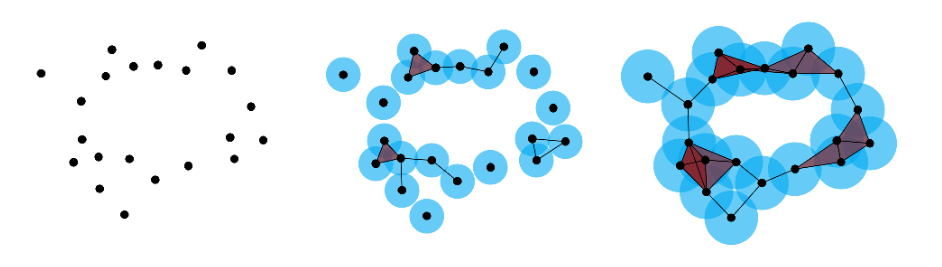
\includegraphics[width=1\textwidth]{images/cech.png}
    \caption{Filtration de cech}
\end{figure}

Il y a beaucoup de blabla sur pourquoi cest une approximation qu'on peut utiliser,
pas compris encore.

A partir d'une filtration, on peut calculer les homologies.

\textbf{Classe d'homologie} : Une classe d'homologie représente un trou dans
qui existe dans le complexe simplicial pour un certain intervalle de filtration.
Classe homologique 0D : un connected component (un trou) (Lespace vide entre
deux connected component)
Classe homologique 1D : un trou qui est borné par un chemin fermé

\textbf{Homologie persistante} : Les informations données par les dates de 
naissance et de mort des classes d'homologie sont appelées homologies persistantes.
Vu que les trous peuvent apparaitre et disparaitre à différentes/indice de 
filtration.

\textbf{Diagramme de persistance} : Un diagramme de persistance est un graphe
qui représente les classes d'homologie en fonction de leur date de naissance
et de mort. Chaque classe d'homologie est représentée par un point dans le
diagramme de persistance.

Citation : we interpret homology classes as holes in coverage
and we interpret the death simplices as the locations of the holes

On peut résumer les informations de l'homologie persistante en un diagramme
de persistance. Un PD est un multi ensemble dans l'espace étentude R^2 
contenant les infinis

\section{Construction des VR complexes massiques}

\section{Construction des objets}

\section{Résultats}
Application sur des villes de France : Paris, Lyon, Marseille, Toulouse.

\section{Conclusion}
Ne tiens pas compte du coûts des infrastructures

\end{document}